\documentclass[hidelinks,12pt]{article}
\usepackage[left=0.25cm,top=1cm,right=0.25cm,bottom=1cm]{geometry}
%\usepackage[landscape]{geometry}
\textwidth = 20cm
\hoffset = -1cm
\usepackage[utf8]{inputenc}
\usepackage[spanish,es-tabla]{babel}
\usepackage[autostyle,spanish=mexican]{csquotes}
\usepackage[tbtags]{amsmath}
\usepackage{nccmath}
\usepackage{amsthm}
\usepackage{amssymb}
\usepackage{mathrsfs}
\usepackage{graphicx}
\usepackage{subfig}
\usepackage{standalone}
\usepackage[outdir=./Imagenes/]{epstopdf}
\usepackage{siunitx}
\usepackage{physics}
\usepackage{color}
\usepackage{float}
\usepackage{hyperref}
\usepackage{multicol}
%\usepackage{milista}
\usepackage{anyfontsize}
\usepackage{anysize}
%\usepackage{enumerate}
\usepackage[shortlabels]{enumitem}
\usepackage{capt-of}
\usepackage{bm}
\usepackage{relsize}
\usepackage{placeins}
\usepackage{empheq}
\usepackage{cancel}
\usepackage{wrapfig}
\usepackage[flushleft]{threeparttable}
\usepackage{makecell}
\usepackage{fancyhdr}
\usepackage{tikz}
\usepackage{bigints}
\usepackage{scalerel}
\usepackage{pgfplots}
\usepackage{pdflscape}
\pgfplotsset{compat=1.16}
\spanishdecimal{.}
\renewcommand{\baselinestretch}{1.5} 
\renewcommand\labelenumii{\theenumi.{\arabic{enumii}})}
\newcommand{\ptilde}[1]{\ensuremath{{#1}^{\prime}}}
\newcommand{\stilde}[1]{\ensuremath{{#1}^{\prime \prime}}}
\newcommand{\ttilde}[1]{\ensuremath{{#1}^{\prime \prime \prime}}}
\newcommand{\ntilde}[2]{\ensuremath{{#1}^{(#2)}}}

\newtheorem{defi}{{\it Definición}}[section]
\newtheorem{teo}{{\it Teorema}}[section]
\newtheorem{ejemplo}{{\it Ejemplo}}[section]
\newtheorem{propiedad}{{\it Propiedad}}[section]
\newtheorem{lema}{{\it Lema}}[section]
\newtheorem{cor}{Corolario}
\newtheorem{ejer}{Ejercicio}[section]

\newlist{milista}{enumerate}{2}
\setlist[milista,1]{label=\arabic*)}
\setlist[milista,2]{label=\arabic{milistai}.\arabic*)}
\newlength{\depthofsumsign}
\setlength{\depthofsumsign}{\depthof{$\sum$}}
\newcommand{\nsum}[1][1.4]{% only for \displaystyle
    \mathop{%
        \raisebox
            {-#1\depthofsumsign+1\depthofsumsign}
            {\scalebox
                {#1}
                {$\displaystyle\sum$}%
            }
    }
}
\def\scaleint#1{\vcenter{\hbox{\scaleto[3ex]{\displaystyle\int}{#1}}}}
\def\bs{\mkern-12mu}


\title{Operadores autoadjuntos \\ \large {Tema 3 - Bases completas y ortogonales}\vspace{-3ex}}

\author{M. en C. Gustavo Contreras Mayén}
\date{ }

\pagestyle{fancy}
\fancyhf{}
\rhead{Curso MAF}
\lhead{\leftmark}
\rfoot{\thepage}
\setlength{\headheight}{16pt}%


\begin{document}
\maketitle
\fontsize{14}{14}\selectfont
\tableofcontents
\newpage

%Ref. Herman (2015) 4.2.1 Adjoint Operators
\section{Operadores autoadjuntos.}

En el estudio de la teoría espectral de matrices, se aprende sobre el adjunto de la matriz, $\vb{A}^{\dagger}$, y el papel que juegan las matrices autoadjuntas o Hermitianas en la diagonalización. Además, se necesita el concepto de \emph{adjunto} para discutir la existencia de soluciones al problema matricial:
\begin{align*}
\vb{y} = \vb{A} \, \vb{x}
\end{align*}

En el mismo sentido, uno está interesado en la existencia de soluciones de la ecuación del operador $L \, u = f$ y soluciones del correspondiente problema de valores propios. El estudio de operadores lineales en un espacio de Hilbert es una generalización de lo que estudia en un curso de álgebra lineal.
\par
Así como se puede encontrar una base de vectores propios y diagonalizar matrices Hermitianas o autoadjuntas (o simétricas reales en el caso de matrices reales), veremos que el operador de Sturm-Liouville es \emph{autoadjunto}. En esta parte definiremos el dominio de un operador e introduciremos la noción de \emph{operadores adjuntos}. Veremos el papel que juega el adjunto en la existencia de soluciones a la ecuación del operador $L \, u = f$.
\par
Comenzamos definiendo el adjunto de un operador: el adjunto, $L^{\dagger}$, del operador $L$ satisface:
\begin{align*}
\langle u, L \, v \rangle = \langle L^{\dagger} \, u,  v \rangle
\end{align*}
para todo $v$ en el dominio de $L$ y $u$ en el dominio de $L^{\dagger}$. Aquí, el dominio de un operador diferencial $L$ es el conjunto de todos $u \in L_{\sigma}^{2} (a, b)$ que satisfacen un conjunto dado de CDF homogéneas. Esto se comprenderá mejor con el siguiente ejemplo.
\par
\noindent
\textbf{Ejemplo 1.} Encuentra el adjunto de:
\begin{align*}
L = a_{2} (x) \, D^{2} + a_{1} (x) \, D + a_{0} (x)
\end{align*}
con $D = \dv*{x}$.
\par
\noindent
Para encontrar el adjunto, colocamos el operador dentro de una integral. Considera el producto interior:
\begin{align*}
\langle u , L \, v \rangle = \scaleint{5ex}_{\bs a}^{b} u (a_{2} \, \sderivada{v} + a_{1} \, \pderivada{v} + a_{0} \, v) \dd{x}
\end{align*}

Tenemos que \enquote{mover} el operador $L$ de $v$ y determinar qué operador está actuando sobre $u$ para preservar formalmente el producto interno. Para un operador simple como $L = \dv*{x}$, esto se hace fácilmente mediante la integración por partes. Para el operador dado, necesitaremos aplicar varias integraciones por partes a los términos individuales. Consideramos cada término derivado en el integrando por separado.
\par
Para el término $a_{1} \, \pderivada{v}$, integramos por partes para encontrar:
\begin{align}
\begin{aligned}[b]
\scaleint{5ex}_{\bs a}^{b} \, u(x) \, a_{1} \, \pderivada{v}(x) \dd{x} &= a_{1}(x) \, u(x) \, v(x) \eval_{a}^{b} + \\[0.5em]
&- \scaleint{5ex}_{\bs a}^{b} \big[ u(x) \, a_{1} (x) \big]^{\prime} \, v(x) \dd{x}
\end{aligned}
\label{eq:ecuacion_04_17}
\end{align}

Ahora consideremos el caso para el término $a_{2} \, \sderivada{v}$, en donde será necesario hacer dos integraciones por partes:
\begin{align}
\begin{aligned}[b]
&\scaleint{5ex}_{\bs a}^{b} \, u(x) \, a_{2} (x) \, \sderivada{v}(x) \dd{x} = a_{2}(x) \, u(x) \, \pderivada{v}(x) \eval_{a}^{b} - \scaleint{5ex}_{\bs a}^{b} \big[ u(x) \, a_{2} (x) \big]^{\prime} \, \pderivada{v}(x) \dd{x} = \\[0.5em]
&= \bigg[ a_{2}(x) \, u(x) \, \pderivada{v}(x) - \big[ a_{2}(x) \, u(x) \big]^{\prime} \, v(x) \bigg] \eval_{a}^{b} + \\[0.5em]
&+ \scaleint{5ex}_{\bs a}^{b} \, \big[ u(x) \, a_{2} (x) \big]^{\prime \prime} \, v(x) \dd{x}
\end{aligned}
\label{eq:ecuacion_04_18}
\end{align}
Combinando estos resultados, tenemos que:
\begin{align}
\begin{aligned}[b]
\langle u , L \, v \rangle &= \scaleint{5ex}_{\bs a}^{b} u (a_{2} \, \sderivada{v} + a_{1} \, \pderivada{v} + a_{0} \, v) \dd{x} = \\[0.5em]
&= \bigg[ a_{1} (x) \, u (x) \, v (x) + a_{2} (x) \, u(x) \, \pderivada{v}(x) - \big[ a_{2} (x) \, u (x) \big]^{\prime} \, v (x) \bigg] \eval_{a}^{b} + \\[0.5em]
&+ \scaleint{5ex}_{\bs a}^{b} \, \big[ u (x) \, a_{2} (x) \big]^{\prime \prime} \, v (x) \dd{x}
\end{aligned}
\label{eq:ecuacion_04_19}
\end{align}

Agregando las CDF para $v$, uno tiene que determinar las CDF para $u$ tales que:
\begin{align*}
\bigg[ a_{1} (x) \, u(x) \, v(x) + a_{2} (x) \, u(x) \, \pderivada{v} (x) - \big[ a_{2} (x) \, u(x) \big]^{\prime} \, v (x) \bigg] \eval_{a}^{b} = 0
\end{align*}
Estos nos lleva a:
\begin{align*}
\langle u , L \, v \rangle &= \scaleint{5ex}_{\bs a}^{b}  \big[ (a_{2} \, u)^{\prime \prime} - (a_{1} \, u)^{\prime} + a_{0} \, u \big] \, v \dd{x} \equiv \langle L^{\dagger} \, u, v \rangle 
\end{align*}
Por lo tanto:
\begin{align}
L^{\dagger} = a_{2} (x) \, \dv[2]{x} - a_{1} (x) \, \dv{x}  + a_{0}(x)
\label{eq:ecuacion_04_20}
\end{align}
Cuando $L^{\dagger} = L$, el operador se llama formalmente \textbf{autoadjunto}, también es conocido como \emph{operador Hermitiano}.
\par
Cuando el dominio de $L$ es el mismo que el dominio de $L^{\dagger}$, se utiliza el término autoadjunto. Como el dominio es importante para establecer el autoadjunto, en el siguiente ejemplo completo se encontrará el dominio del adjunto.
\\[0.5em]
\noindent
\textbf{Ejemplo 2.} Determina $L^{\dagger}$ y su dominio para el operador:
\begin{align*}
L \, u = \dv{u}{x}
\end{align*}
donde $u$ satisface las CDF $u(0) = 2 \, u(1)$ en $[0, 1]$.

Necesitamos encontrar el operador adjunto que satisfaga \hfill \break $\langle v, L \, u \rangle = \langle L^{\dagger} \, v, u \rangle$. Por lo que reescribimos la integral:
\begin{align*}
\langle v, L \, u \rangle = \scaleint{5ex}_{\bs 0}^{1} v \, \dv{u}{x} \dd{x} = u \, v \eval_{0}^{1} - \scaleint{5ex}_{\bs 0}^{1} u \, \dv{v}{x} \dd{x} = \langle L^{\dagger} \, v, u \rangle
\end{align*}
De esto tenemos el problema adjunto que consiste en un operador adjunto y la CDF asociada (o dominio de $L^{\dagger}$):
\begin{enumerate}
\item $L^{\dagger} = - \displaystyle \dv{x}$
\item $\displaystyle u \, v \eval_{0}^{1} = 0 \Rightarrow u(1) \big[ v(1) - 2 \, v(0) \big] \Rightarrow v(1) = 2 \, v(0)$
\end{enumerate}
\vspace{0.3cm}
\noindent
%Ref. Arfken (2006) 10.2.1
% \textbf{Ejercicio a cuenta (30).} Las funciones $\phi_{1}(x)$ y $\phi_{2}(x)$ son funciones propias del mismo operador autoadjunto (Hermitiano) pero para distintos valores propios $\lambda_{1}$ y $\lambda_{2}$. Demuestra que $\phi_{1}(x)$ y $\phi_{2}(x)$ son linealmente independientes.

\section{Identidades de Lagrange y de Green.}

Antes de pasar a la demostración de que los valores propios de un problema de Sturm-Liouville son reales y las funciones propias asociadas son ortogonales, primero necesitaremos introducir dos identidades importantes. Para el operador de Sturm-Liouville:
\begin{align*}
\mathcal{L} = \dv{x} \left( p \, \dv{x} \right) + q
\end{align*}
se tienen dos identidades:
\\
\noindent
\textbf{Identidad de Lagrange:} 
\begin{align*}
u \, \mathcal{L} \, v - v \, \mathcal{L} \, u = \big[ p \, (u \, \pderivada{v} - v \, \pderivada{u}) \big]^{\prime}
\end{align*}
\noindent
\textbf{Identidad de Green:} 
\begin{align*}
\scaleint{5ex}_{\bs a}^{b} \, \big(u \, \mathcal{L} \, v - v \, \mathcal{L} \, u \big) \dd{x} = \big[ p \, (u \, \pderivada{v} - v \, \pderivada{u}) \big]\eval_{a}^{b}
\end{align*}

La prueba de la identidad de Lagrange sigue una sencilla manipulación del operador:
\begin{align}
\begin{aligned}[b]
u \, \mathcal{L} \, v - v \, \mathcal{L} \, u &= u \bigg[ \dv{x} \left( p \dv{v}{x} \right) + q \, v \bigg] - v \bigg[ \dv{x} \left( p \dv{v}{x} \right) + q \, u \bigg] = \\[0.5em]
&= u \dv{x} \left( p \dv{v}{x} \right) - v \dv{x} \left( p \dv{u}{x} \right) = \\[0.5em]
&= u \dv{x} \left( p \dv{v}{x} \right) + p \dv{u}{x} \dv{v}{x} - v \dv{x} \left( p \dv{u}{x} \right) - p \dv{u}{x} \dv{v}{x} = \\[0.5em]
&= \dv{x} \bigg[ p \, u \, \dv{v}{x} - p \, v \, \dv{u}{x}  \bigg]
\end{aligned}
\label{eq:ecuacion_04_21}
\end{align}
La identidad de Green se prueba simplemente integrando la identidad de Lagrange.

\newpage

\section{Ortogonalidad y valores reales.}

Ahora estamos listos para demostrar que \emph{los valores propios de un problema de Sturm-Liouville son reales y que las funciones propias correspondientes son ortogonales}. Esto se revisa fácilmente utilizando la identidad de Green, que a su vez es una declaración de que el operador de Sturm-Liouville es autoadjunto.
\\
\noindent
\textbf{Ejemplo 3.} Los valores propios del problema de tipo Sturm-Liouville son reales, este ejercicio se presentó en las  notas anteriores:
\begin{align*}
\mathcal{L} \, y = \left( x \, \pderivada{y} \right)^{\prime} + \dfrac{2}{x} \, y = - \lambda \, \sigma \, y
\end{align*}

Sean las $\phi_{n}(x)$ una solución para el problema de valores propios asociados con $\lambda_{n}$:
\begin{align*}
\mathcal{L} \, \phi_{n} = - \lambda_{n} \, \sigma \, \phi_{n}
\end{align*}
Mostrando que $\overline{\lambda}_{n} = \lambda_{n}$, donde la barra significa el conjugado complejo\footnote{En algunos textos para denotar el conjugado complejo, se ocupa un asterisco como superíndice, en este ejemplo la notación sería: $\lambda_{n}^{*} = \lambda_{n}$}. Entonces, también consideramos el conjugado complejo de esta ecuación:
\begin{align*}
\mathcal{L} \, \overline{\phi}_{n} = - \overline{\lambda}_{n} \, \sigma \, \overline{\phi}_{n}
\end{align*}
Multiplicando la primera ecuación por $\overline{\phi}_{n}$, la segunda ecuación por $\phi_{n}$ y luego restando los resultados, obtenemos:
\begin{align*}
\overline{\phi}_{n} \, \mathcal{L} \, \phi_{n} - \phi_{n} \, \mathcal{L} \, \overline{\phi}_{n} = \big( \overline{\lambda}_{n} - \lambda_{n} \big) \, \sigma \, \phi_{n} \, \overline{\phi}_{n}
\end{align*}
integrando ambos lados de la expresión, se llega a:
\begin{align*}
\scaleint{5ex}_{\bs a}^{b} \bigg( \overline{\phi}_{n} \, \mathcal{L} \, \phi_{n} - \phi_{n} \, \mathcal{L} \, \overline{\phi}_{n} \bigg) \dd{x} = \big( \overline{\lambda}_{n} - \lambda_{n} \big) \, \scaleint{5ex}_{\bs a}^{b} \sigma \, \phi_{n} \, \overline{\phi}_{n} \dd{x}
\end{align*}
aplicando la identidad de Green en el lado izquierdo, se tiene que:
\begin{align*}
\big[ p \, (u \, \pderivada{v} - v \, \pderivada{u}) \big]\eval_{a}^{b} = \big( \overline{\lambda}_{n} - \lambda_{n} \big) \, \scaleint{5ex}_{\bs a}^{b} \sigma \, \phi_{n} \, \overline{\phi}_{n} \dd{x}
\end{align*}

Usando las condiciones homogéneas:
\begin{align*}
\alpha_{1} \, y(a) + \beta_{1} \, \ptilde{y} (a) &= 0 \\[0.5em]
\alpha_{2} \, y(b) + \beta_{2} \, \ptilde{y} (b) &= 0
\end{align*}
para el operador autoadjunto, el lado izquierdo se anula. Por lo que el resultado es:
\begin{align*}
\big( \overline{\lambda}_{n} - \lambda_{n} \big) \, \scaleint{5ex}_{\bs a}^{b} \sigma \, \norm{\phi_{n}}^{2} \dd{x} = 0
\end{align*}
esta integral es no negativa, por lo que se tiene $\overline{\lambda}_{n} = \lambda_{n}$. Entonces los valores propios son reales.
\\
\noindent
\textbf{Ejemplo 4.} Las funciones propias correspondientes a diferentes valores propios de un problema tipo Sturm-Liouville son ortogonales.
\begin{align*}
\dv{x} \left( p(x) \, \dv{x} \right) + q(x) \, y + \lambda \, \sigma (x) \, y = 0
\end{align*}

La demostración es similar al ejemplo anterior. Sea $\phi_{n}(x)$ una solución al problema de valores propios con $\lambda_{n}$:
\begin{align*}
\mathcal{L} \, \phi_{n} = - \lambda_{n} \, \sigma \, \phi_{n}
\end{align*}
y sea $\phi_{m}(x)$ una solución al problema de valores propios asociado con \hfill \break $\lambda_{m} \neq \lambda_{n}$:
\begin{align*}
\mathcal{L} \, \phi_{m} = - \lambda_{m} \, \sigma \, \phi_{m}
\end{align*}
Ahora, multiplicamos la primera ecuación por $\phi_{m}$ y la segunda ecuación por $\phi_{n}$. Restando estos resultados, obtenemos:
\begin{align*}
\phi_{m}\, \mathcal{L} \, \phi_{n} - \phi_{n} \, \mathcal{L} \, \phi_{m} = \big( \lambda_{m} - \lambda_{n} \big) \, \sigma \, \phi_{n} \, \phi_{m}
\end{align*}
integrando ambos lados de la ecuación, usando la identidad de Green y usando las CDF homogéneas, se tiene:
\begin{align*}
\big( \lambda_{m} - \lambda_{n} \big) \, \scaleint{5ex}_{\bs a}^{b} \sigma \, \phi_{n} \, \phi_{m} \dd{x} = 0
\end{align*}
dado que los valores propios son distintos, podemos dividir entre $\lambda_{m} - \lambda_{n}$, llegando al resultado deseado:
\begin{align*}
\scaleint{5ex}_{\bs a}^{b} \sigma \, \phi_{n} \, \phi_{m} \dd{x} = 0
\end{align*}
Por lo tanto, las funciones propias son ortogonales con respecto a la función de peso $\sigma(x)$.
\par
Puede presentarse el caso en el que las funciones propias no sean ortogonales, en la siguiente sección se revisa el procedimiento que garantiza que siempre será posible contar con una ortogonalización de funciones.

\section{Ortogonalización de Gram-Schmidt.}

Este método toma un conjunto de funciones (o vectores) no ortogonales linealmente dependientes y genera un conjunto ortogonal de funciones (o vectores) en un intervalo arbitrario con respecto a una función de peso arbitraria.
\par
Las funciones involucradas pueden ser reales o complejas, por conveniencia, asumiremos que las funciones son reales, la generalización para funciones complejas, no ofrece mayor dificultad.
\par
Veamos el caso de la normalización de funciones, que implica lo siguiente:
\begin{align*}
\scaleint{5ex}_{\bs a}^{b} \phi_{i}^{2} \, \sigma  \, \dd{x}  =  N_{i}^{2}
\end{align*}
revisemos que no se le ha puesto atención al valor de $N_{i}$. Ya que la ecuación básica 
\begin{align}
\mathcal{L} \, u(x) + \lambda \, \sigma(x) \, u(x) = 0
\label{eq:ecuacion_10_08}
\end{align}
es lineal y homogénea, podemos multiplicar la solución por cualquier constante, de tal manera que sigue siendo solución. Por lo que podemos pedir que tal solución $\phi_{i}(x)$ se multiplique por $N_{i}^{-1}$ y ahora la nueva $\phi_{i}$ (normalizada) $\phi_{i}$ satisface:
\begin{align}
\scaleint{5ex}_{\bs a}^{b} \, \phi_{i}^{2} (x) \, \sigma(x) \, \dd{x} = 1
\label{eq:ecuacion_10_39}
\end{align}
o en términos de una delta:
\begin{align}
\scaleint{5ex}_{\bs a}^{b} \, \phi_{i}(x) \, \phi_{j} (x) \, \sigma (x) \, \dd{x} = \delta_{ij}
\label{eq:ecuacion_10_40}
\end{align}
La ecuación (\ref{eq:ecuacion_10_39}) nos dice que hemos normalizado a la unidad; incluyendo la propiedad de ortogonalidad, tenemos la ecuación (\ref{eq:ecuacion_10_40}), las funciones que las satisfacen, se dice que son \textbf{ortonormales} (ortogonales y normalizadas), cabe señalar que existen otras formas de normalización, cada una de las funciones especiales de la Física Matemática se puede normalizar de distintas formas.
\par
Consideremos tres conjuntos de funciones:
\begin{enumerate}
\item Un conjunto original, linealmente independiente $u_{n}(x)$ con $n=0,1,2,\ldots$ \\
Las funciones podrían ser funciones propias degeneradas, pero no es necesario que se cumpla este punto.
\item Un conjunto ortogonal $\psi_{n}(x)$ que se va a construir.
\item Un conjunto de funciones $\phi_{n}(x)$ que será normalizadas $\psi_{n}(x)$
\end{enumerate}
Tendremos las siguientes propiedades:
\begin{center}
{\fontsize{12}{12}\selectfont
\renewcommand{\arraystretch}{1.5}%
\begin{tabular}{p{4.5cm} p{4.5cm} p{4.5cm}}
\hline
\makecell{$u_{n}(x)$} & \makecell{$\psi_{n}(x)$} & \makecell{$\phi_{n}(x)$} \\ \hline
\makecell{linealmente \\ independiente} &    \makecell{linealmente \\ independiente} & \makecell{linealmente \\ independiente} \\ \hline
\makecell{no ortogonal} & \makecell{ortogonal} & \makecell{ortogonal} \\ \hline
\makecell{no normalizada} & \makecell{no normalizada} & \makecell{normalizada \\ (ortonormal)} 
\end{tabular}
}
\end{center}

\subsection{La técnica de ortogonalización.}

La técnica de Gram-Schmidt consiste en tomar la n-ésima función $\psi$ ($\psi_{n}$) para ser $u_{n}(x)$ más un combinación lineal no conocida de la función $\phi$ previa. El que haya una nueva $u_{n}(x)$ nos dará la garantía de que se mantenga la independencia lineal.
\par
El que $\psi_{n}(x)$ sea ortogonal para cada $\phi$ previa, apenas nos da elementos para determinar los coeficientes desconocidos. Así cuando ya se determine $\psi_{n}$, se normaliza a la unidad, dejando $\phi_{n}(x)$. Este procedimiento se repite para las $\psi_{n+1}(x)$.

Empezamos con $n = 0$, sea:
\begin{align}
\psi_{0} = u_{0}(x)
\label{eq:ecuacion_10_41}
\end{align}
no nos preocupemos al no tener una $\phi$ previa. Entonces normalizamos:
\begin{align}
\phi_{0}(x) = \dfrac{\psi_{0}(x)}{\left[ \displaystyle \scaleint{5ex} \psi_{0}^{2} \, \sigma  \, \dd{x} \right]^{1/2}}
\label{eq:ecuacion_10_42}
\end{align}
Para $n = 1$, tenemos:
\begin{align}
\psi_{1}(x) = u_{1}(x) + a_{1,0} \, \phi_{0}(x)
\label{eq:ecuacion_10_43}
\end{align}
Que requiere que $\psi_{1}(x)$ sea ortogonal a $\phi_{0}(x)$ (en este punto, la normalización de $\psi_{1}(x)$ es irrelevante). La ortogonalidad nos conduce a:
\begin{align}
\scaleint{5ex} \psi_{1} \, \phi_{0} \, \sigma \, \dd{x} = \scaleint{5ex} u_{1} \, \phi_{0} \, \sigma \, \dd{x} + a_{1,0} \scaleint{5ex} \phi_{0}^{2} \, \sigma \dd{x} = 0
\label{eq:ecuacion_10_44}
\end{align}
Ya que $\phi_{0}$ se normaliza a la unidad (ec. \ref{eq:ecuacion_10_42}), tenemos:
\begin{align}
a_{1,0} = - \scaleint{5ex} u_{1} \, \phi_{0} \, \sigma \dd{x}
\label{eq:ecuacion_10_45}
\end{align}
fijando el valor de $a_{1, 0}$. Normalizando, definimos:
\begin{align}
\phi_{1} (x) = \dfrac{\psi_{1}(x)}{\left( \displaystyle \scaleint{5ex} \psi_{1}^{2} \, \sigma \dd{x} \right)^{1/2}}
\label{eq:ecuacion_10_46}
\end{align}
Generalizando, resulta:
\begin{align}
\phi_{i}(x) = \dfrac{\psi_{i}(x)}{\left( \displaystyle \scaleint{5ex} \psi_{i}^{2}(x) \, \sigma (x) \dd{x} \right)^{1/2}}
\label{eq:ecuacion_10_47}
\end{align}
donde:
\begin{align}
\psi_{i}(x) = u_{i} + a_{1, 0} \, \phi_{0} + a_{i, 1} \, \phi_{1} + \ldots + a_{i, i-1} \, \phi_{i-1}
\label{eq:ecuacion_10_48}
\end{align}
Los coeficientes $a_{i, j}$ están dados por
\begin{align}
a_{i, j} = - \scaleint{5ex} u_{i} \, \phi_{j} \, \sigma  \dd{x}
\label{eq:ecuacion_10_49}
\end{align}
La ecuación (\ref{eq:ecuacion_10_49}) es para una normalización unitaria. Para otros tipos de normalización, se tiene que:
\begin{align*}
\scaleint{5ex}_{\bs a}^{b} \left[ \phi_{j} (x) \right]^{2} \, \sigma (x) \dd{x} =  N_{j}^{2}
\end{align*}
Entonces la ecuación (\ref{eq:ecuacion_10_47}) se reemplaza por:
\begin{align}
\phi_{i}(x) =  N_{i} \: \dfrac{\psi_{i}(x)}{\left( \displaystyle \scaleint{5ex} \psi_{i}^{2} \, \sigma \dd{x} \right)^{1/2}}
\label{eq:ecuacion_10_47a}
\end{align}
y los términos $a_{i,j}$ resultan:
\begin{align}
a_{i, j} = - \dfrac{ \displaystyle \scaleint{5ex} u_{i} \, \phi_{j} \, \sigma \dd{x}}{N_{j}^{2}}
\label{eq:ecuacion_10_49a}
\end{align}
% Las ecuaciones (\ref{eq:ecuacion_10_48}) y (\ref{eq:ecuacion_10_49}) pueden escribirse en términos de operadores de proyección $P_{j}$. Si consideramos que $\phi_{n}(x)$ forman un espacio vectorial lineal, la integral en la ecuación \ref{eq:ecuacion_10_49}) puede interpretarse como la proyección de $u_{i}$ en la \enquote{coordenada} $\phi_{j}$ o la componente $j$-ésima de $u_{i}$. Con:
% \begin{align*}
% P_{j} \, u_{i}(x) = \left[ \scaleint{5ex} u_{i}(t) \, \phi_{j}(t) \, \sigma(t) \dd{t} \right]\, \phi_{j}(x)
% \end{align*}
% la ecuación (\ref{eq:ecuacion_10_48}) resulta ahora:
% \begin{align}
% \psi_{i}(x) = \left\{ 1 - \nsum_{j=1}^{i-1} P_{j} \right\} \, u_{i}(x)
% \label{eq:ecuacion_10_48a}
% \end{align}
% Restando los $j-$-ésimos componentes: $j = 1$ a $i - 1$, resulta que $\psi_{i}(x)$ es ortogonal para todo $\phi_{j}(x)$.
% \par

Cabe señalar que el procedimiento de Gram-Schmidt es una manera de construir un conjunto ortogonal o ortonormal, pero las funciones $\phi_{i}(x)$ no son únicas. Existe un infinito de posibles conjuntos ortonormales para un intervalo dado y una función de peso dada.
\\[0.5em]
\noindent
\textbf{Ejemplo 4. } \texttt{Ortogonalización de Gram-Schmidt para los polinomios de Legendre.}

Queremos generar un conjunto ortonormal\footnote{Toma en cuenta que aunque se indican algunas expresiones como integrales, se presenta el resultado pero no el procedimiento para obtener ese valor, tienes la libertad de realizar las operaciones y comprobar efectivamente que se logra ese resultado.} a partir de las funciones: 
\begin{align*}
u_{n}(x) = x^{n}, \hspace{1.5cm} n = 0, 1, 2, \ldots
\end{align*}
El intervalo es $-1 \leq x \leq 1$ y la función de peso es $\sigma (x) = 1$.
\par
De acuerdo a la técnica descrita de ortogonalización de Gram-Schmidt:
\begin{align}
u_{0} (x) = 1 \hspace{1.5cm} \phi_{0} (x) =  \dfrac{1}{\sqrt{2}}
\label{eq:ecuacion_10_50}
\end{align}
Entonces:
\begin{align}
\psi_{1}(x) = x + a_{1,0} \, \dfrac{1}{\sqrt{2}}
\label{eq:ecuacion_10_51}
\end{align}
donde:
\begin{align}
a_{1, 0} = - \scaleint{5ex}_{\bs -1}^{1} \dfrac{x}{\sqrt{2}} \, \dd{x} = 0
\label{eq:ecuacion_10_52}
\end{align}
por simetría. Normalizando $\psi_{1}$, obtenemos:
\begin{align}
\phi_{1}(x) = \sqrt{\dfrac{3}{2}} \, x
\label{eq:ecuacion_10_53}
\end{align}
Continuando el método de Gram-Schmidt, se define ahora:
\begin{align}
\psi_{2} (x) = x^{2} +  a_{2, 0} \, \dfrac{1}{\sqrt{2}} +  a_{2, 1} \, \sqrt{\dfrac{3}{2}} \, x
\label{eq:ecuacion_10_54}
\end{align}
donde:
\begin{align}
a_{2, 0} &= - \scaleint{5ex}_{\bs -1}^{1} \, \dfrac{x^{2}}{\sqrt{2}} \, \dd{x} = - \dfrac{\sqrt{2}}{3} \label{eq:ecuacion_10_55} \\[1em] 
a_{2, 1} &= - \scaleint{5ex}_{\bs -1}^{1} \, \sqrt{\dfrac{3}{2}} \, x^{3} \dd{x} = 0 \label{eq:ecuacion_10_56}
\end{align}
de nueva cuenta por simetría. Por tanto:
\begin{align}
\psi_{2}(x) = x^{2} - \dfrac{1}{3}
\label{eq:ecuacion_10_57}
\end{align}
normalizando a la unidad, tenemos:
\begin{align}
\phi_{2} (x) = \sqrt{\dfrac{5}{2}} \, \dfrac{1}{2} \, (3 \, x^{2} - 1)
\label{eq:ecuacion_10_58}
\end{align}
La siguiente función $\phi_{3}(x)$ es:
\begin{align}
\phi_{3} (x) = \sqrt{\dfrac{7}{2}} \, \dfrac{1}{2} \, (5 \, x^{3} - 3 \, x)
\label{eq:ecuacion_10_59}
\end{align}
Se puede demostrar que:
\begin{align}
\phi_{n}(x) = \sqrt{\dfrac{2 \, n + 1}{2}} \, P_{n}(x)
\label{eq:ecuacion_10_60}
\end{align}
donde $P_{n}$ es el polinomio de Legendre\footnote{El uso de funciones especiales como en este caso los polinomios de Legendre $P_{n}(x)$, será algo común, ya en el Tema 5 se revisará la construcción completa de los $P_{n}(x)$, así como un conjunto de propiedades.} de orden $n$.
% \\[0.5em]
% \noindent
% \textbf{Ejercicio a cuenta (31). } Considera los siguientes elementos:
% \begin{enumerate}[label=\alph*)]
% \item Un conjunto de funciones $\left\{ u_{n} (x) \right\} = \left\{ x^{n} \right\}, \mbox{ con } n = 1, 2, \ldots$
% \item El intervalo $(0, \infty)$
% \item Una función de peso $\sigma (x) = x \, e^{-x}$
% \end{enumerate}
% Con el método de Gram-Schmidt construye las primeras \textbf{tres funciones ortonormales} del conjunto $u_{n}(x)$, con ese intervalo dado y función de peso dada.

\section{Polinomios ortogonales.}
\subsection{Conjunto de polinomios.}

El ejemplo anterior se ha elegido estrictamente para ilustrar el procedimiento de Gram-Schmidt. Aunque tiene la ventaja de introducir los polinomios de Legendre, las funciones iniciales $u_{n} = x^{n}$ no son funciones propias degeneradas y no son soluciones de la ecuación de Legendre. Son simplemente un conjunto de funciones que hemos reorganizado aquí para crear un conjunto ortonormal para el intervalo dado y la función de peso dada. El hecho de que hayamos obtenido los polinomios de Legendre no es \enquote{magia negra}, sino una consecuencia directa de la elección de la función de peso y del intervalo.
\par
El uso de $u_{n} (x) = x^{n}$ pero eligiendo otros intervalos y funciones de peso, nos conduce a otros conjuntos de polinomios ortogonales, como se muestra en la tabla (\ref{tabla:tabla_03}):
\begin{landscape}
\begin{table}[H]
\centering
{\renewcommand{\arraystretch}{1.5}%
%\resizebox{\textwidth}{!}{%
\begin{tabular}{p{5cm} c c p{10cm}}
\hline
\makecell{Polinomios} & Intervalo & $\sigma (x)$ & \makecell{Normalización estándar} \\ \hline
Legendre & $ -1 \leq x \leq 1$ & $1$ & $\displaystyle \scaleint{5ex}_{\bs -1}^{1} \left[ P_{n}(x) \right]^{2} \dd{x} = \dfrac{2}{2 \, n + 1} $ \\
Legendre desplazados & $ 0 \leq x \leq 1$ & $1$ & $\displaystyle \scaleint{5ex}_{\bs -1}^{1} \left[ P_{n}^{*}(x) \right]^{2} \dd{x} = \dfrac{2}{2 \, n + 1} $ \\
Chebyshev tipo I & $-1 \leq x \leq 1$ & $(1 - x^{2})^{-1/2}$ & $\displaystyle \scaleint{5ex}_{\bs -1}^{1} \dfrac{\left[ T_{n}(x) \right]^{2}}{(1 - x^{2})^{-1/2}} \dd{x} = \begin{cases} 
\displaystyle \frac{\pi}{2} & n \neq 0 \\
\pi & n = 0 \end{cases} $ \\
Chebyshev desplazados I & $0 \leq x \leq 1$ & $[x (1 - x)]^{-1/2}$ & $\displaystyle \scaleint{5ex}_{\bs -1}^{1} \dfrac{\left[ T_{n}^{*} (x) \right]^{2}}{[x (1 - x)]^{-1/2}} \dd{x} = \begin{cases} 
\displaystyle \frac{\pi}{2} & n > 0 \\
\pi & n = 0 \end{cases} $ \\
Chebyshev II & $-1 \leq x \leq 1$ & $(1 - x^{2})^{1/2}$ & $\displaystyle\scaleint{5ex}_{\bs -1}^{1} [U_{n} (x)]^{2} \, (1 - x^{2})^{1/2} \, \dd x = \frac{\pi}{2}$ \\
Laguerre & $0 \leq x < \infty $ & $e^{-x}$ & $\displaystyle \scaleint{5ex}_{\bs 0}^{\infty} \left[ L_{n} (x) \right]^{2} \, e^{-x} \dd{x} =  1 $ \\
Asociados de Laguerre & $0 \leq x < \infty $ & $x^{k} \, e^{-x}$ & $\displaystyle \scaleint{5ex}_{\bs 0}^{\infty} \left[ L_{n}^{k} (x) \right]^{2} \, x^{k} \, e^{-x} \dd{x} = \dfrac{(n + k)!}{n!} $ \\
Hermite & $- \infty < x < \infty $ & $e^{-x^{2}}$ & $\displaystyle \scaleint{5ex}_{\bs -\infty}^{\infty} \left[ H_{n} (x) \right]^{2} e^{-x^{2}} \dd{x} = 2^{n} \, \pi^{1/2} \, n! $
\end{tabular}}
\caption{Polinomios ortogonales generados por la ortogonalización de Gram-Schmidt de $u_{n} (x)= x^{n}$, con $n=0,1,2,\ldots$}
\label{tabla:tabla_03}
\end{table}
\end{landscape}
Una revisión de este proceso de ortogonalización revelará dos características arbitrarias:
\begin{enumerate}
\item Primero, como se enfatizó antes, no es necesario normalizar las funciones a la unidad. En el ejemplo que acabamos de dar, podríamos haber requerido:
\begin{align}
\scaleint{5ex}_{\bs -1}^{1} \phi_{n} (x) \: \phi_{m} (x) \, \dd{x} = \dfrac{2}{2 \, n +1} \, \delta_{nm}
\label{eq:ecuacion_10_61}
\end{align}
y el conjunto resultante habría el de los polinomios de Legendre.
\item Segundo, el signo de $\phi_{n} (x)$ siempre es indeterminado. En el ejemplo, elegimos el signo al requerir que el coeficiente de mayor potencia de $x$ en el polinomio sea positivo. Para los polinomios de Laguerre, por otro lado, requeriríamos que el coeficiente de mayor potencia sea $(-1)^{n}/n!$
\end{enumerate}
% \vspace*{0.5cm}
%Ref. Arfken (2006) 10.3.9
% \textbf{Ejercicio a cuenta (32). } Forma un conjunto ortogonal en el intervalo $0 \leq x < \infty$ usando $u_{n} = \exp(-n \, x), n = 1, 2, 3, \ldots$, usa la función de peso $\sigma(x) = 1$. Esas funciones son soluciones a la EDO2H:
% \begin{align*}
% \sderivada{u}_{n} - n^{2} \, u_{n} = 0
% \end{align*}
% la cual se revisa directamente que es de la forma de tipo Sturm-Liouville (autoadjunta). ¿Por qué la teoría de Sturm-Liouville no garantiza la ortogonalidad de estas funciones?

\section{Problema de valores propios.}

\begin{ejemplo}
Resuelve el problema de tipo Sturm-Liouville:

\begin{align*}
x^{2} \, \sderivada{y} + 5 \, x \, \pderivada{y} + \lambda \, y = 0
\end{align*}
con las condiciones:
\begin{align*}
y(1) = y(e) = 0 \hspace{1.5cm} 1 \leq x \leq e
\end{align*}

Resolver el ejercicio implica obtener:
\begin{enumerate}
\item Los correspondientes eigenvalores.
\item La eigenfunciones.
\item Revisar la ortogonalidad de éstas.
\end{enumerate}

Tomemos en cuenta que la forma de esta ecuación es:
\begin{align*}
a_{2} (x) \, \sderivada{y} + a_{1} (x) \, \pderivada{y} + a_{0}(x) \, y + \lambda \, y = f(x)
\end{align*}
se tiene que:
\begin{align*}
a_{2} (x) = x^{2}, \hspace{0.5cm} a_{1} (x) = 5\, x, \hspace{0.5cm} a_{0} (x) = 0
\end{align*}

Recordemos que la forma de tipo Sturm-Liouville es:
\begin{align*}
\dv{x} \left( p(x) \, \dv{x} \right) \, y + q(x) \, y + \lambda \, \sigma (x) \, y = 0
\end{align*}
donde:
\begin{align*}
p (x) &= \dfrac{1}{a_{2} (x)} \, \exp \left( \scaleint{5ex} \, \dfrac{a_{1} (x)}{a_{2} (x)} \dd{x} \right) \\[0.5em] 
q (x) &= p (x) \, \dfrac{a_{0} (x)}{a_{2} (x)} \hspace{1.5cm} F (x) = p (x) \, \dfrac{f (x)}{a_{2} (x)}
\end{align*}
Entonces:
\begin{align*}
p(x) &= \dfrac{1}{a_{2}(x)} \exp \left( \scaleint{5ex} \dfrac{a_{1}(x)}{a_{2}(x)} \dd{x} \right) = \\[0.5em] 
&= \dfrac{1}{x^{2}} \, \exp \left( \scaleint{5ex} \dfrac{5 x}{x^{2}} \dd{x} \right) = \\[0.5em] 
&= \dfrac{1}{x^{2}} \,  \exp \left( 5 \, \scaleint{5ex} \, \dfrac{1}{x} \dd{x} \right) = \\[0.5em] 
&= \dfrac{1}{x^{2}} \,  \exp \left( 5 \, \ln x \right) =  x^{3} > 0 \hspace{0.2cm} \mbox{en } 1 \leq x \leq e
\end{align*}

Se tiene además que:
\begin{align*}
q(x) = 0 \hspace{1.5cm} F(x) = 0
\end{align*}
Por lo que la EDO en forma de tipo Sturm-Liouville es:
\begin{align*}
\dv{x} \big( x^{5} \, \pderivada{y} \big) + \lambda \, x^{3} \, y = 0
\end{align*}

El problema es de tipo autoadjunto (Hermitiano), ya que las CDF son homogéneas. En consecuencia, los eigenvalores son reales y las eigenfunciones son ortogonales.
\par
La ecuación que debemos de resolver es:
\begin{align*}
x^{2} \, \sderivada{y} + 5 \, x \, \pderivada{y} + \lambda \, y = 0
\end{align*}

Identificamos que es una ecuación de tipo Euler, con $y(x) = x^{m}$. La ecuación característica es:
\begin{align*}
m^{2} + 4 \, m + \lambda = 0
\end{align*}
entonces:
\begin{align*}
m = - 2 \pm \sqrt{4 - \lambda}
\end{align*}

La solución general de la EDO es:
\begin{align*}
y (x) = \dfrac{1}{x^{2}} \, \left( a \, x^{\sqrt{4 - \lambda}} + b \, x^{- \sqrt{4 - \lambda}} \right)
\end{align*}

De las CDF, se tiene que $y (1) = 0$,  entonces $b = -a$, así:
\begin{align*}
y (x) = \dfrac{a}{x^{2}} \, \left( x^{\sqrt{4 - \lambda}} + x^{- \sqrt{4 - \lambda}} \right)
\end{align*}

Con la condición $y(e) = 0$, se tienen dos casos:
\begin{enumerate}[label=\roman*)]
\item Si $4 - \lambda > 0$
\begin{align*}
\Rightarrow \hspace{0.3cm} \sinh \sqrt{4 - \lambda} &= 0 \\[0.5em]  
\lambda &= 4
\end{align*}
Por tanto $y (x) = 0$
\item Si $4 - \lambda < 0$
\begin{align*}
\Rightarrow \hspace{0.3cm} \sen \sqrt{4 - \lambda} &= 0 \\[0.5em]  
\sqrt{\lambda - 4} &= n \, \pi \\[0.5em] 
\lambda &= 4 + n^{2} \, \pi^{2}
\end{align*}
\end{enumerate}

La solución general se expresa como:
\begin{align*}
y (x) = \dfrac{a}{x^{2}} \left( x^{i n \pi} - x^{-i n \pi} \right)
\end{align*}
considerando que $x = e^{\ln x}$, tendremos:
\begin{align*}
y (x) &= \dfrac{a}{x^{2}} \bigg[ \exp \big( i \, n \, \pi \, \ln x \big) -  \exp \big( - i \, n \, \pi \, \ln x \big) \bigg] = \\[0.5em] 
&= \dfrac{a}{x^{2}} \, 2 \, i \, \sin (n \, \pi \, \ln x)
\end{align*}

El conjunto de eigenvalores es:
\begin{align*}
\left\{ \lambda_{n} \right\} = 4 + n^{2} \, \pi^{2}
\end{align*}
{
\def\arraystretch{1}
\begin{tabular}{c c}
$\lambda_{1} =$ & $13.8696$ \\
$\lambda_{2} =$ & $43.4784$ \\
$\lambda_{3} =$ & $92.8264$ \\
$\lambda_{4} =$ & $161.914$ \\
$\vdots$
\end{tabular}}

El conjunto de las eigenfunciones es:
\begin{align*}
\left\{ y_{n} (x) \right\} = \left\{ \dfrac{1}{x^{2}} \sin (n \, \pi \, \ln x) \right\}
\end{align*}
Tomemos en cuenta que las funciones aún no están normalizadas.
\par
Revisando la ortogonalidad:
\begin{align*}
&\scaleint{5ex}_{\bs x=1}^{x=e} \, p (x) \, y_{n}^{*} (x) \, y_{m}(x) \dd{x} = \\[0.5em] 
&= \scaleint{5ex}_{\bs x=1}^{x=e} \, \dfrac{1}{x} \, \sin (n \, \pi  \, \ln x) \, \sin (m \, \pi  \, \ln x) \dd{x}
\end{align*}

Haciendo el cambio de variable, tal que $x = e^{u}$, entonces:
\begin{itemize}
\item  Si $m \neq n$:
\begin{align*}
\scaleint{5ex}_{\bs 0}^{1} \, \sin (n \, \pi  \, u) \, \sin (m \, \pi  \, u) \dd{u} = 0
\end{align*}
\item Si $m = n$, se tiene que:
\begin{align*}
\scaleint{5ex}_{\bs x=1}^{x=e} \, p(x) \, y_{n}^{2} (x) \dd{x} = \dfrac{\pi}{2}
\end{align*}
\end{itemize}

El conjunto de eigenfunciones normalizadas, con la función de peso $p(x) = x^{3}$ en el intervalo $1 \leq x \leq e$ es:
\begin{align*}
\left\{ y_{n} (x) \right\} = \left\{ \sqrt{\dfrac{2}{\pi}} \, \dfrac{\sin (n \, \pi \, \ln x)}{x^{2}} \right\}
\end{align*}

Aunque el enunciado del problema no lo indique, conviene presentar una gráfica de las eigenfunciones obtenidas, tal como se presenta a continuación:
\begin{figure}[H]
    \centering
    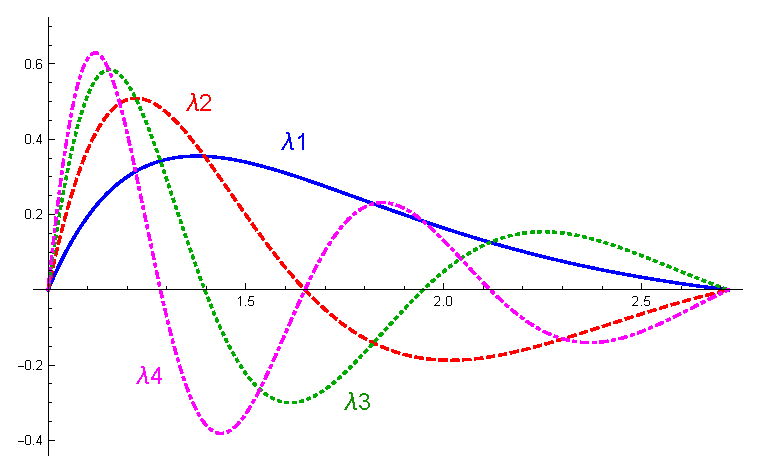
\includegraphics[scale=0.85]{Imagenes/Ejercicio_SL_01_Funciones.eps}
    \caption{Gráfica de las primeras eigenfunciones con sus correspondientes eigenvalores.}
    \label{fig:figura_}
\end{figure}
\end{ejemplo}
\end{document}